\documentclass{life-en}
\usepackage{eurosans}
\usepackage{totpages}

\begin{document}

\title{La Vie est un Jeu}
\subtitle{User's Guide}
\member{Lepage Barbara}{lepage.barbara@gmail.com}
\member{Caradec Guillaume}{guillaume.caradec@gmail.com }
\member{Corsin Simon}{simoncorsin@gmail.com }
\member{Glorieux François}{fra.glorieux@gmail.com}
\member{Klarman Nicolas}{nickoas@gmail.com}
\member{Lassagne David}{david.lassagne@gmail.com}
\member{Louvigny Guillaume}{guillaume@louvigny.fr}
\member{El-Outmani Youssef}{youssef.eloutmani@gmail.com}
\member{Le-Cor Wilfried}{wilfried.lecor@gmail.com}
\member{Lenormand Frank}{lenormf@gmail.com}

\summary
{
	In this document, you'll be able to discover the several features
	of our project 
}

\maketitle
\authorspage

%% --------------------------------------------------------------------- %%

\chapter*{Document's informations}

\rowcolors{1}{white}{lightgray}
\begin{tabular}{ | m{5cm} | m{10cm} | }
	\hline
	\textbf{Document Type} & User Documentation\\ % to change
	\hline
	\textbf{Complete document name} & «~La Vie Est Un Jeu~», the User's guide\\ % to change
	\hline
	\textbf{Keywords} & «~User~», «~Tutorial~», «~conception~», «~lavieestunjeu~»\\ % to change
	\hline
	\textbf{Number of pages} & \ref{TotPages} \\
	\hline
	\textbf{Group's name} & La Vie Est Un Jeu\\
	\hline
	\textbf{Responsible} & Group's leader : Barbara Lepage\\
	\hline
	\textbf{Contact} & lavieestunjeu@googlegroups.com\\
	\hline
	\textbf{Revision} & 1.0\\ % to change
	\hline
	\textbf{Development Website} & \url{http://eip.epitech.eu/2014/lavieestunjeu/}\\
	\hline
	\textbf{Official Website} Not Available yet.\\
	\hline
\end{tabular}

\newpage

\tableofcontents

%% --------------------------------------------------------------------- %%

\chapter{Introduction and context}

\section{«~La Vie Est Un Jeu~»}

\subsection{«~La vie est un Jeu~», is not just yet another basic social network !}

There are already existing solutions in terms of Social Network but we'd like to create our own kind with the idea of entertainment associated. \\
\\
That's why you will find in «LIFE» what could be compared to a list of the «must have done things». This list is not unique, actually the choice belongs to you, you define it ! What is important to achieve in your life ? You tell me ! This way, we allow you to share to your friends/family/whatever what really matters to you.\\
\\
Each entry in the system (Activity/achivement completed or failed etc..) will be open to your friends for comments. In these slots, you'll be able to share any
media (pictures/videos etc) or simply discuss about the current achivement/activity.\\
\\
We thought that this innovative side for social networks seemed to be ommited, so here's the occasions for you fans of challenge to keep a trace of the differents actions you've accomplished and an occasion to meet persons sharing the same passion !\\
\\

%% --------------------------------------------------------------------- %%

\section{Project's Vocabulary}

\subsection{What's an «~achievement~» ?}
The term achievement comes from the video-games world, it's a series of goals/actions that need to be done to unlock differents rewards. It's not related to the main objective (which is in most cases to beat the final boss or finish the main quest).\\
\\
Achivements are a way to distinguish a player from another one when they've both finished a game. These achievements also increase the in-game challenge and the gamelife's duration.\\
\\
According to several sources, a player feels rewarded and happy when it comes to unlock achievements. Game designers also use them to make 
the player discover several sides of the game he would have probably avoided without their presence.\\
\\
The fact that you can share your successes with your friends would probably make them want to take their revenge try to do better than what you did.
That's why we think that's an interesting thing to do an analogy between games and life.\\
\\

Depending on the successes you'll unlock (and thanks to the categories they belong to), the system will be able to classify your interests and you as interesting for other users. This way, we hope than you'll meet 
people sharing the same passions and will be encouraged to go further into this passion.\\


%% --------------------------------------------------------------------- %%

\subsection{Project's ease of use.}

For you guys, the final users, our project is made of a website and several mobile applications on systems including Android, iOs and Windows Phone. If you're willing to use our project as a developper, we'll setup a public API allowing to bring developpers' creativity. We hope that several services will see the light !

The different features we wanted in our project weren't present or combined in the several existing solutions. This project is our attempt to give you a platform that you'll visit on a daily basis without neglecting discussions and media sharing.

\newpage

\subsection{Projet's Aim}

We want to create users' communities around an achievement's system directly linked to real daily life, whether topic of interests or professional life.\\
\\
In theory, there's no special target : Everyone has hobbies, passions and topics of interest.\\
\\
The website and the applications are aimed to handle multi-languages, so you're not limited to your own country.

% --------------------------------------------------------------------- %%

\chapter{Details about Website and SmartPhone applications}

\section{The website}

\subsection{Overview of the welcome page, before login}

You will see one of the thousand available achievements (Probably the most popular classified by publication date) and the diverse features. This diaporama is attracting, isn't it ? What are you waiting for ? Let's create an account, it's easy, fast and free !\\
\\
The subscription is detailled later in this document.
If you're already into the system, this page will allow you to sign in.\\
\\
We could also put a system to browse the different achiements' categories and their achievements to allow non signed-in users have an overview of what's feasible within our project.

\newpage

\subsection{Subscription, the first five minutes}

We wanted this step to be a light one because sometimes you're confronted to a heavy form which is not attrative.
That's why you could find our innovative way to handle your subscription step by step allowing you to discover our tool and its universe as you get through these different steps.\\
\\
You'll often be asked to answer simple questions to complete your public profile during your following visits. This way, we combine a guide and user's subscriptions without being too annoying. These questions will be simple enough to be answere almost directly.\\
\\
\begin{figure}[H]
	\begin{center}
		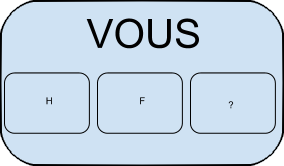
\includegraphics[width=10cm]{img/vous.png}
	\end{center}
\end{figure}

\subsection{User's main page}

You can retrieve the activities that are available in your stream here. It's been done in a Facebook/Google+-like manner.\\

There are 4 subsections available through the menu :
\begin{itemize}
	\item Your stream (Default Page) ;
	\item Your objectives ;
	\item Your achievements ;
	\item Your «friends» (imported from others social network or added through our website).
\end{itemize}

A « breaking news » bar will always be on top on the website to show the last official news and the activities of your friends.

\begin{figure}[H]
	\begin{center}
		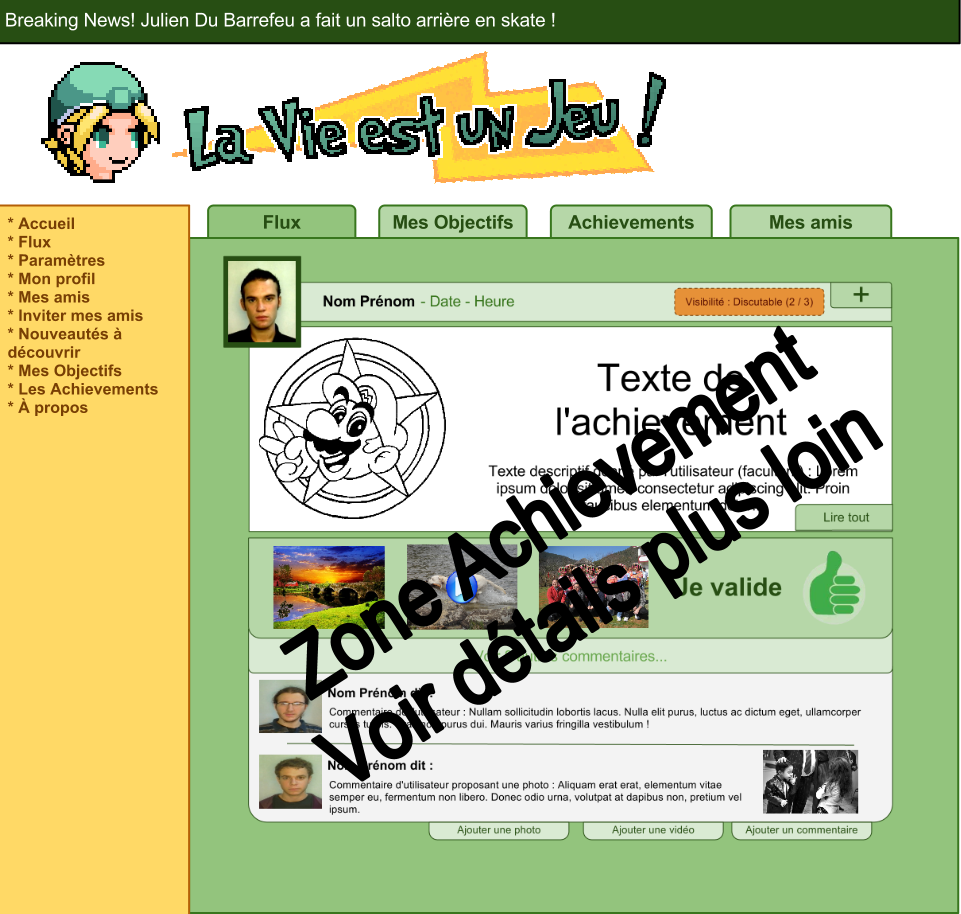
\includegraphics[width=15cm]{img/accueil.png}
	\end{center}
\end{figure}


\subsection{Your stream}

The stream is on the middle of the main page and its role is to display the last activities of your friends and the different publication in a semi-detailled way.

It will contain :
\begin{itemize}
	\item The « achievements » to be validated;
	\item The objectives that your friends chose ;
	\item New friendships / contacts ;
	\item Official news (informations or new achievements).
\end{itemize}

\newpage

\subsection{Achievements}

You'll be able to pick achievements' packs containing several achievements through this page. Each pack is classified by theme so they coul be ranked to match your preferences and interests.\\
\\
You can then mark some of the challenges to be your current/futures objectives which will notify your circle.

\subsection{Achievement's details}

Each achievement will be validable as the commentaries/publication are in Facebook/Google+ (The «like» and «+1» buttons). This way, you'll be able to notify the content's owner that you find it interesting. You can also discuss about it and give feedbacks to the creator.\\
\\
The «Plus» button is aimed to show the whole set of commentaries about this achievement in order to avoid data overloading.\\

\begin{figure}[H]
	\begin{center}
		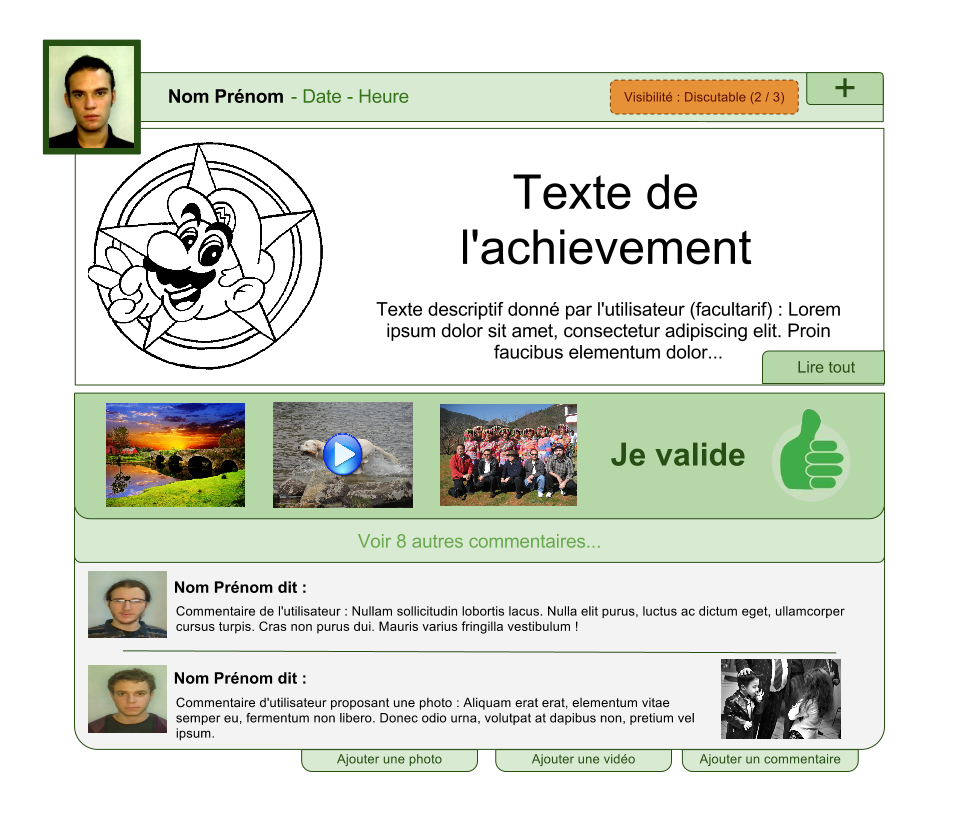
\includegraphics[width=15cm]{img/achievement.png}
	\end{center}
\end{figure}

\subsection{Objectives}
In this page, the aim is to let you create your custom objectives' list in order to mark the achivements you're wiling to unlock in the near future. It's also from thi page that you can mark an objective as completed.\\

\subsection{Contacts}

In this page, you can browse your contacts' lists and organize them into users groups. It allows you to define authorized/forbidden contents on a per-group basis.\\
\\
There are 4 levels of access you can define and this feature is aimed to prevent other users accessing something that belong to your private life if you don't want them to access it.\\
\\
Please find further explanations on this content limitation later in the document.

\subsection{Groups}

Also known as communities, these groups are created to put togethers achievements, medias, publications and users that belong to a certain category (For example : Computer Science / Football etc..)\\
\\
You can list these groups and join them from this page. By joining groups, you will be able to get new special achievements but also a chance to contribute to the groups by giving your ideas about new challenges/opinions on current ideas.\\
\\
In groups there are several levels of access : You can request to be moderator if you deserve it !
These moderators are in charge of :
\\
\begin{itemize}
\item Check that the users' behaviors are conform to what's expected in the rules
\item Validate or not the differents submissions (Achivement ideas / Publications)
\item Directly add content into database
\end{itemize}

The third user category in groups is the owners, they are responsible of the moderators' management. They can add/remove moderator status in order to delegate tasks.\\
\\
If you don't find an existing group matching your expectations, don't hesitate to create your own ! It will be useful for other users.

\subsection{Profile}

The Profile page holds data about a user and allow him to modify these informations. It also provides a way for other users to interact with this user :
\begin{itemize}
\item Message sending
\item Request to join friends' circle
\end{itemize}

You can also find the different rewards the user has unlocked and click on it to view the details of the differents achievements (Type, action requested and commentaries/medias associated etc)
\\
\section{Smartphone application}

For the smartphones' applications, we have chosen to use internet views to develop an interface based on the technology we're using in the website (Ocsigen).\\
\\

So it shouldn't be fundamentally different on the several supports, please read the website documentations and you'll be fine :).

\section{API}

If you're willing to develop a specific service using our API, please find the specific document for the API, it's available on the website at this link. (Not written yet)

\end{document}
